\chapter{Language server}

The purpose of Language server is to implement the Language Server Protocol and Debug Adapter Protocol and to provide access to parser library using these protocols. It has to deserialize and serialize LSP and DAP messages, keep them in the right order and then serve all the requests by invoking parser library.

\section{LSP}
short overview of LSP

definition of message, notification, request
\section{DAP}
short overview of DAP

\section{Third party libraries}
Language server uses three third party libraries: ASIO C++ library \footnote{\url{https://think-async.com/Asio/}}, JSON for Modern C++ \footnote{\url{https://github.com/nlohmann/json}} and 
cpp-netlib URI \footnote{\url{https://github.com/cpp-netlib/uri}}.

\subsection{ASIO C++ library}
Asio is a cross-platform C++ library for network and low-level I/O programming that provides developers with a consistent asynchronous model using a modern C++ approach. We use it to handle TCP communication in a cross-platform way. Asio implements std::iostream wrappers around the TCP stream, which allows us to abstract from the actual source of the communication.

\subsection{JSON for Modern C++}
We use the JSON for Modern C++ library to parse and serialize json, it is used in both LSP and DAP. It allows us to seamlessly traverse input json and extract the interesting values as well as easily respond with valid json messages.

\subsection{cpp-netlib URI}
Cpp-netlib URI library supports URI specified by the RFC3986 \footnote{\url{https://tools.ietf.org/html/rfc3986}}, which is used by the LSP and DAP protocols to transfer paths to files. It is the responsibility of language server to parse the URIs and convert them to file paths, so it is easier to work with them in the parser library. 

\section{Language server overview}
The architecture of the Language server component is illustrated in \cref{lang_server_arch}. It communicates on standard input/output by LSP with LSP client and listens on a TCP port to provide DAP support for macro tracer. The TCP communication is wrapped by class \TT{TCP handler}, which uses boost::asio library to provide the TCP communication as common C++ iostream.


\begin{figure}
	\centering
	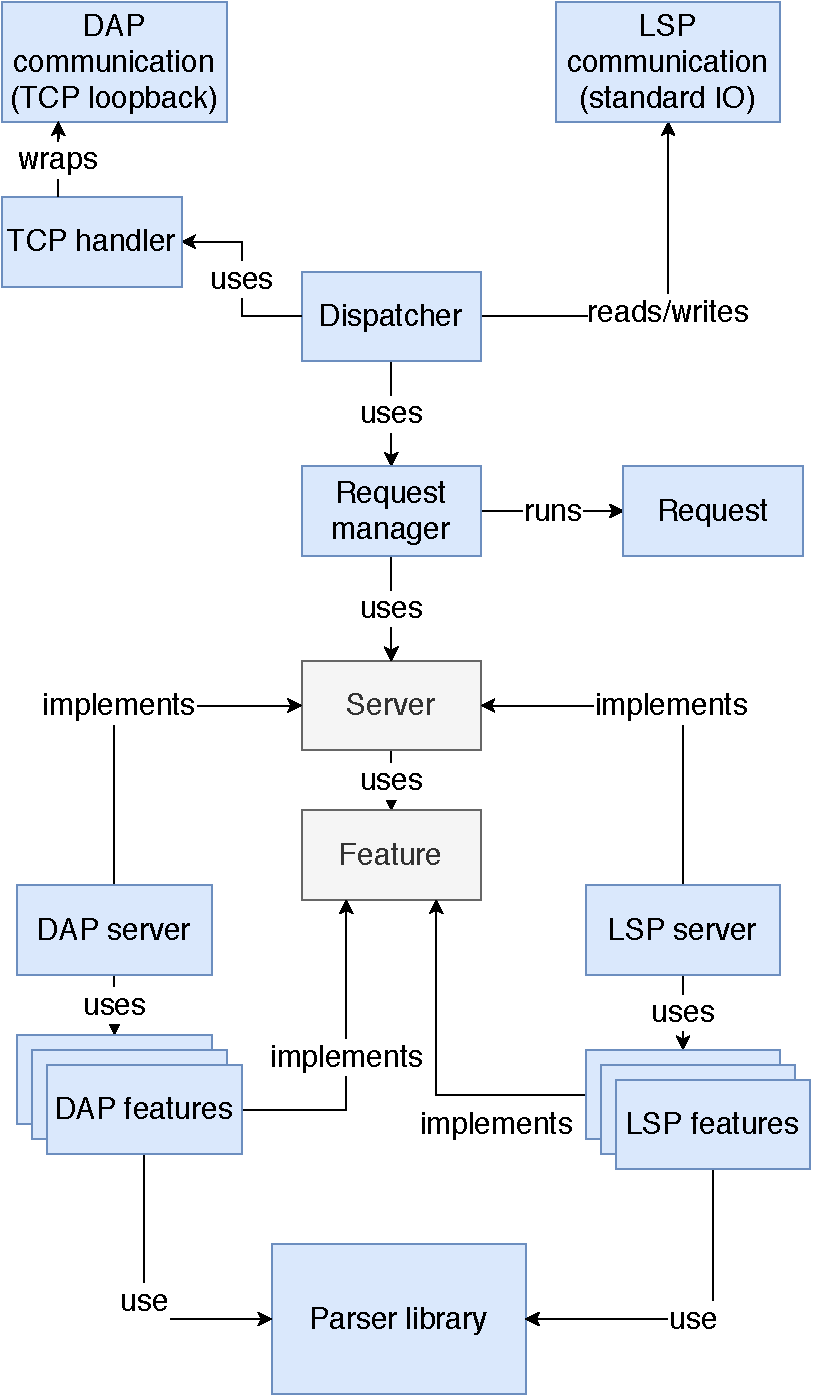
\includegraphics[width=11cm]{img/lang_server}
	\caption{Architecture of language server.}
	\label{lang_server_arch}
\end{figure}


The main purpose of the \TT{Dispatcher} is to provide abstraction for the lowest level communication, which is shared by LSP and DAP. It reads iostream to parse messages using the JSON for Modern C++ library and stores them in \TT{request manager} as requests.

A \TT{request} encapsulates one message that came from the client and basically is represented only by raw (but parsed) json.

\TT{Request manager} stores \TT{requests} in a queue and runs a worker thread that serves the requests one by one. There is only one instance of request manager running in the language server, so it serializes requests from DAP and LSP (which come asynchronously from separate sources) into one queue.

\TT{Server} is an abstract class that implements protocol behaviour that is common for both DAP and LSP - it basically implements Remote Procedure Call. Actual handling of LSP and DAP requests is implemented in \TT{features}. Each \TT{feature} contains implementation of several protocol requests or notifications. The \TT{features} unwrap the arguments from json and call corresponding parser library methods.

Both LSP and DAP have their implementation of the abstract \TT{server} class. They both implement the beginning and end of protocol communication, which is a bit different for both protocols and both use \TT{features} to serve protocol requests.


\section{Dispatcher}
\TT{Dispatcher} main task is to read from and write into the input/output stream and abstract from the complexity of reading raw strings from streams. Its output is a message that consist of parsed message.

- parses input, the same for lsp and dap


\section{Server}
abstract class that basically implements RPC






implementations: 
\subsection{LSP server}
-lsp\_server
\subsection{DAP server}
-dap\_server
\section{Request Manager}


